% ============================================================================
% JINS Special Issue Manuscript
% ============================================================================
\documentclass[11pt,a4paper]{article}

% --- Geometry and formatting ---
\usepackage[margin=2.5cm, headheight=14pt]{geometry}
\usepackage[utf8]{inputenc}
\usepackage[T1]{fontenc}
\usepackage{mathpazo}
\usepackage{setspace}
\setstretch{1.25}

% --- Tables and figures ---
\usepackage{booktabs}
\usepackage{tabularx}
\usepackage{multirow}
\usepackage{graphicx}
\graphicspath{{figures/}}
\usepackage{float}
\usepackage{caption}
\usepackage{subcaption}
\captionsetup{font=small, labelfont=bf}

% --- Math and symbols ---
\usepackage{amsmath}
\usepackage{amssymb}
\usepackage{textcomp}

% --- Colors and hyperlinks ---
\usepackage{xcolor}
\definecolor{clinteal}{RGB}{0,119,182}
\definecolor{clinred}{RGB}{213,94,0}
\definecolor{clinamber}{RGB}{230,159,0}
\definecolor{clingreen}{RGB}{0,158,115}
\newif\ifshowrevisions
\showrevisionsfalse
\newcommand{\revblue}[1]{\ifshowrevisions\textcolor{blue}{#1}\else#1\fi}
\usepackage[colorlinks=true,linkcolor=clinteal,citecolor=clinteal,urlcolor=clinteal]{hyperref}

% --- Microtypography ---
\usepackage{microtype}

% --- Lists ---
\usepackage{enumitem}

% --- Headers ---
\usepackage{fancyhdr}
\pagestyle{fancy}
\fancyhf{}
\renewcommand{\headrulewidth}{0pt}
\rfoot{\thepage}

% --- Bibliography ---
\usepackage[style=apa,backend=biber,natbib=true]{biblatex}
\addbibresource{jins_references.bib}
\setlength{\bibhang}{1.5em}
\setlength{\bibitemsep}{0.45\baselineskip}

% --- TikZ for pipeline diagrams ---
\usepackage{tikz}
\usetikzlibrary{shapes.geometric, arrows.meta, positioning, fit, calc, backgrounds}

% --- Author block ---
\usepackage{authblk}

% --- Suppress section numbering (APA style) ---
\setcounter{secnumdepth}{0}

% ============================================================================
\begin{document}

% --- Title ---
\begin{center}
{\Large\bfseries An AI-Initiated, Rule-Based Pipeline for Pre-Examination Screening in Clinical Neuropsychology}

\bigskip

% --- Authors ---
Astri J.\ Lundervold\textsuperscript{a,*},\quad
Birgitte Berentsen\textsuperscript{b},\quad
Arvid Lundervold\textsuperscript{c,d}

\medskip

{\small
\textsuperscript{a}Department of Clinical and Biological Psychology, University of Bergen, Bergen, Norway\\
\textsuperscript{b}National Centre for Functional Gastrointestinal Disorders, Department of Medicine, Haukeland University Hospital, Bergen, Norway\\
\textsuperscript{c}Department of Biomedicine, University of Bergen, Bergen, Norway\\
\textsuperscript{d}Mohn Medical Imaging and Visualization Centre (MMIV), Department of Radiology, Haukeland University Hospital, Bergen, Norway\\[4pt]
\textsuperscript{*}Corresponding author: \href{mailto:astri.lundervold@uib.no}{astri.lundervold@uib.no}\\[4pt]
ORCID: Astri J.\ Lundervold \href{https://orcid.org/0000-0002-6819-6164}{0000-0002-6819-6164};\quad
Birgitte Berentsen \href{https://orcid.org/0000-0003-3574-7078}{0000-0003-3574-7078};\\
Arvid Lundervold \href{https://orcid.org/0000-0002-0032-4182}{0000-0002-0032-4182} {\tiny v. 2026-03-27; 2026-04-09; 2026-04-13}
}
\end{center}

\bigskip

% ============================================================================
\begin{abstract}
\noindent
\textbf{Objective.} We present a proof-of-concept framework for automated pre-examination screening in clinical neuropsychology. The long-term vision is a tool that receives digitalized screening data before the patient's first visit, enabling the clinician to plan a tailored examination. As fully digital instruments are not yet universally available, the framework is demonstrated on existing data from a study of irritable bowel syndrome (IBS). A deterministic pipeline automates the synthesis, transforming multi-domain scores into a structured clinical analysis with cross-domain reasoning and audience-tailored reports.

\textbf{Method.} The pipeline processes five instruments (Bergen Insomnia Scale, Conners' CPT-3, Chalder Fatigue Scale, Hospital Anxiety and Depression Scale, and the Repeatable Battery for the Assessment of Neuropsychological Status [RBANS]), applying published cutoffs for questionnaire and CPT measures, and using RBANS data for both index-score group comparisons and cohort-relative patient-level summaries. 
For each patient it generates an eight-step rule-based reasoning chain, cohort-contextualized visualizations, and PDF reports in three variants for clinical peers, referring physicians, and patients. Revised analyses were performed on an analysis-ready cohort dataset comprising 105 adults (65 IBS, 40 healthy controls) from the Bergen Brain--Gut--Microbiota study. 
The pipeline was co-developed with an AI coding assistant during development, including Claude Opus 4.6, and GPT-5.4; however, no AI is used at runtime.

\textbf{Results.} The pipeline identified flagged findings in sleep (50\%), fatigue (40\%), anxiety (35\%), and attention (30\%), with multi-domain flags in 60\%. Cross-domain reasoning chains linked co-occurring findings to plausible mechanisms (e.g., insomnia--fatigue--attention cascades). Two case illustrations demonstrated differentiated clinical formulations across diverse profiles.

\textbf{Conclusions.} The framework augments rather than replaces clinical judgment, and its transparent, reproducible architecture supports professional oversight. Full realization depends on the ongoing digitalization of cognitive assessment instruments for remote administration.
\end{abstract}

\medskip
\noindent\textbf{Keywords:} clinical decision support, automated screening, cross-domain reasoning, precision neuropsychology, audience-tailored reporting

\bigskip

% ============================================================================
\section{Introduction}
\label{sec:introduction}

In outpatient neuropsychological practice, clinicians often begin their pre-examination preparation with a referral letter and a set of intake questionnaires that must be synthesized into a clinically meaningful picture of the patient's difficulties and likely needs. This synthesis requires forming preliminary hypotheses about which cognitive, emotional, and functional domains are most relevant, whether interactions across domains are likely to affect test performance, and which aspects of the examination should be prioritized. This work is often done under time pressure and with limited opportunity for systematic review. As a result, clinically relevant patterns may be overlooked, and the examination may default to a standard battery rather than being tailored to the individual patient. More broadly, neuropsychologists must balance clinical productivity with precision in patient care while integrating complex multi-domain information, tailoring assessments to the individual patient, and preparing reports that are both clinically accurate and understandable to others. Report writing itself remains a major workload burden, often requiring two to ten hours per patient depending on report length and patient complexity \citep{Postal2018ReportWriting}. In this setting, tools that can support efficiency while preserving clinical precision are naturally of interest.

This helps explain why artificial intelligence has become increasingly relevant to neuropsychology. In a recent perspective article, \textcite{LundervoldAJ2025} proposed the framework of \textit{precision neuropsychology}, within which incorporating AI into practice presents both opportunities and risks. Used carefully and ethically, AI may help reduce clinician workload, improve access to services, and extend aspects of neuropsychological care to underserved populations \citep{Kronenberger2025}. At the same time, such use must remain transparent, clinically grounded, and subject to professional oversight so that computational support strengthens rather than displaces clinical judgment \citep{LundervoldAJ2025, DeRightPuente2026}.

Despite broader advances in medical AI \citep{Thirunavukarasu2023, Meskó2023}, relatively few concrete changes in everyday neuropsychological practice can be attributed directly to AI adoption \citep{DeRightPuente2026}. Existing applications have mainly focused on computerized testing, automated scoring, and diagnostic classification \citep{Parsons2018Tech, Andersen2026ROCF}. These developments are useful for organizing scores and findings, but they do not address the interpretive task at the center of neuropsychological work: bringing cognitive, emotional, and functional findings together into a coherent clinical formulation. In addition, neuropsychological reports must be tailored to the differing needs of patients and referral sources \citep{Postal2018ReportWriting}.

This leaves an important gap between what automated systems can calculate and what clinicians need before meeting the patient. In practice, the neuropsychologist must consider not only whether a domain is elevated, but also how findings relate to one another and which aspects of the examination deserve particular attention. Support at this stage therefore requires more than score reporting. It requires a structured way of relating findings across domains so that screening data can inform examination planning in a clinically meaningful way.

IBS provides a useful context for examining this challenge. It is a common functional gastrointestinal disorder affecting approximately 14\% of the global population and associated with chronic abdominal pain, altered bowel habits, and reduced quality of life \citep{Arif2025IBS}. Through the gut--brain axis \citep{Mayer2015, Cryan2019}, IBS may also be linked to sleep disturbance \citep{Tu2017}, fatigue \citep{Han2016}, emotional symptoms such as anxiety and depression \citep{Zamani2019}, and more subtle cognitive difficulties \citep{Kennedy2012, Billing2024}. Because these difficulties often co-occur and may influence one another, IBS offers a clinically relevant context for examining how multi-domain screening data may be integrated before formal assessment. In the present study, this question is examined using data from the Bergen Brain--Gut--Microbiota study \citep{Berentsen2020}, and the data set presented in the present study overlaps with data analyzed in prior work on psychological distress subgroups in this cohort \citep{LundervoldAJ2024}. Both that study and a subsequent analysis \citep{LundervoldA2026} have shown considerable overlap in neuropsychological profiles between IBS patients and healthy controls, making the full cohort a useful testbed across a broad range of symptom profiles.

In this study, we present a fully automated, deterministic pipeline as a proof-of-concept framework for pre-examination screening in outpatient neuropsychological practice. Using five established instruments covering sleep, fatigue, emotional distress, sustained attention, and neurocognitive function, the pipeline applies published cutoffs together with cohort-based interpretive rules to generate a structured clinical overview, visual summaries, and report-ready outputs. It is intended as decision support for the pre-examination phase rather than as an autonomous diagnostic system, and the clinician retains full responsibility for diagnostic and therapeutic conclusions.

% ============================================================================
\section{Method}
\label{sec:methods}

\subsection{Participants}

The cohort comprises $N = 105$ adults: 65 patients meeting Rome IV criteria for IBS and 40 age- and gender-matched healthy controls (HC). Participants were recruited through the National Centre for Functional Gastrointestinal Disorders at Haukeland University Hospital, Bergen, Norway, as part of the Bergen Brain--Gut--Microbiota (B-BGM) study \citep{Berentsen2020}. Inclusion criteria for IBS patients required an Irritable Bowel Syndrome Severity Scoring System (IBS-SSS) score $\geq 175$, corresponding to at least moderate symptom severity \citep{Francis1997IBSSSS}. All participants provided written informed consent. The study was approved by the Regional Committee for Medical and Health Research Ethics, South East Norway (REK2015-01621).

All analyses were performed on an analysis-ready cohort file derived from the source dataset after documented data cleaning, while the raw source file was preserved unchanged. The cleaning decisions are documented in the project repository.

Demographic characteristics are summarized in Table~\ref{tab:demographics}. The IBS group included three subtypes: IBS-D (diarrhea-predominant, $n = 24$), IBS-C (constipation-predominant, $n = 9$), and IBS-M (mixed, $n = 32$). IBS symptom severity was assessed using the IBS-SSS (range 0--500; available for $n = 56$ IBS patients), with a mean of $M = 273.8$ ($SD = 71.3$).

\subsection{Neuropsychological instruments}

Five assessment domains were evaluated using established instruments with known psychometric properties. The instruments differ in their administration requirements, which has direct implications for how much of the screening profile can be collected before the patient's first clinic visit. Three self-report questionnaires, the Bergen Insomnia Scale (BIS), Chalder Fatigue Scale (Chalder), and Hospital Anxiety and Depression Scale (HADS), can be administered digitally and completed by patients remotely. The Conners' Continuous Performance Test, Third Edition (CPT-3), is self-administered but currently requires proprietary software on a clinic computer, restricting it to in-clinic use. The Repeatable Battery for the Assessment of Neuropsychological Status (RBANS) requires administration by a trained psychometrician. Thus, in the current landscape, the questionnaire data can arrive before the consultation, while the cognitive test data require an initial clinic-based session:

\begin{enumerate}[leftmargin=*, label=\arabic*.]
    \item \textbf{Sleep/Insomnia -- Bergen Insomnia Scale (BIS)} \textit{[self-report]:} Six items scored 0--7 (days/week), total 0--42 \citep{Pallesen2008}. Pipeline cutoffs: Minimal ($\leq 6$), Mild (7--14), Moderate (15--24), Severe ($\geq 25$); clinical flags at total $\geq 19$ or $\geq 3$ items at $\geq 3$ days/week.

    \item \textbf{Sustained attention -- Conners' CPT-3} \textit{[self-administered, clinic-based]:} A 14-minute continuous performance test yielding T-scored metrics ($M = 50$, $SD = 10$) including Detectability (d$'$), Omissions, Commissions, and Hit Reaction Time \citep{Conners2014}. Pipeline thresholds: T $\geq 60$ (mildly elevated), T $\geq 65$ (clinically significant).

    \item \textbf{Fatigue -- Chalder Fatigue Scale} \textit{[self-report]:} Eleven items with bimodal scoring (0--11) covering physical and mental fatigue \citep{Chalder1993}. Pipeline caseness threshold: $\geq 4$.

    \item \textbf{Emotional distress -- HADS} \textit{[self-report]:} Anxiety (HADS-A) and Depression (HADS-D) subscales, each 0--21 \citep{Zigmond1983}. Pipeline cutoffs: Normal ($\leq 7$), Borderline (8--10), Clinical ($\geq 11$) \citep{Bjelland2002}.

    \item \textbf{Neurocognition -- RBANS} \textit{[clinician-administered]:} Ten subtests assessing the five standard cognitive domains (Immediate Memory, Visuospatial/Constructional, Language, Attention, Delayed Memory) were administered by a trained psychometrician in approximately 30 minutes using the Norwegian version \citep{Randolph2013NO}. In the pipeline, raw RBANS subtests are standardized within the cohort and averaged into domain summary composites aligned with these five domains, while recognition scores are retained as an auxiliary summary and \texttt{RBANS\_Sum\_Raw} is used as a broad total-score indicator. Cognitive flags are raised for marked cohort-relative weakness (domain-summary or total-score percentile $< 16$).
\end{enumerate}

\noindent
The CPT-3 and RBANS are retained as separate domains because they assess complementary aspects of cognition: the CPT-3 targets sustained attention and response inhibition, while the RBANS covers broad cognitive function. Their separation also enables the reasoning engine to distinguish differential patterns (e.g., isolated sustained attention deficits driven by fatigue vs.\ broader cognitive involvement).


\subsection{The deterministic pipeline}

\subsubsection{Architecture overview}

The deterministic pipeline is implemented as a standalone Python program that combines a quantitative analysis layer with structured clinical reasoning. The pipeline was applied to the analysis-ready cohort file described above. Cleaning decisions that required source verification were not overwritten at runtime. Instead, the upstream files preserved the recorded values together with explicit flags, allowing downstream interpretation to remain conservative and auditable.

\paragraph{Clarification on the role of AI.}
During development, the pipeline was co-authored with an AI coding assistant (Cursor IDE with Claude Opus 4.6 and GPT-5.4); all AI-generated content was reviewed, verified, and edited by the authors. At runtime, however, \textbf{no AI is involved}: the deployed pipeline contains no LLM API calls, no AI client libraries, and no network dependencies. All clinical classifications, reasoning chains, and recommendations are produced by deterministic, rule-based logic operating on published cutoffs and pre-authored text templates (Supplementary Material~S1). In short, AI was used to \textit{author the rules}; the rules themselves execute deterministically without AI.

The pipeline processes each patient through five sequential stages:

\begin{enumerate}[leftmargin=*, label=(\roman*)]
    \item \textbf{Data ingestion and preprocessing:} Loading the analysis-ready cohort file, computing derived scores (BIS total, Chalder bimodal total, HADS total), and validating score ranges. Upstream cleaning standardizes datatypes, missing-value encoding, and selected metadata labels while preserving unresolved discrepancies as flagged values rather than silently correcting them.

    \item \textbf{Per-domain analysis:} For each of the five domains, the pipeline applies established clinical cutoffs to generate severity classifications and identify clinically significant findings. For the self-report instruments (BIS, Chalder, HADS), cutoffs are applied directly to raw or derived sum scores. For CPT-3, the pipeline uses software-generated T-scores and interprets higher values as less favorable across the selected metrics; Detectability, Omissions, Commissions, HRT, HRT SD, Perseverations, and Variability are flagged at $T \geq 60$/$T \geq 65$. For RBANS, the pipeline uses cohort-standardized raw subtests rather than age-corrected index columns, with a total raw-score composite retained as a broad overall indicator. Cognitive flags are raised for marked cohort-relative weakness (domain-summary or total-score percentile $< 16$). Because missingness is handled on a domain-specific basis, the effective denominator varies across measures.

    \item \textbf{Cross-domain pattern analysis:} A rule-based engine identifies co-occurring elevations across domains and generates mechanistic hypotheses. For example, elevated BIS combined with low cohort-relative RBANS memory summaries triggers hypotheses about impaired sleep-dependent memory consolidation, whereas co-occurring HADS anxiety elevation with CPT decrements triggers hypotheses about anxiety-related attentional interference. The full set of cross-domain rules is documented in Supplementary Material~S1.

    \item \textbf{Eight-step clinical reasoning chain:} A structured protocol designed to mirror the integrative reasoning used in clinical neuropsychological interpretation (Figure~\ref{fig:reasoning_chain}; example content in Table~\ref{tab:reasoning_chain}). Step~1 establishes demographic and clinical context. Steps~2--6 assess each domain independently: sleep (BIS), fatigue (Chalder), emotional distress (HADS), sustained attention (CPT), and neurocognition (RBANS). Step~7 integrates findings across domains, identifying co-occurring patterns and formulating mechanistic hypotheses. Step~8 synthesizes the integrated profile into a prognostic formulation. The full reasoning-chain specification is provided in Supplementary Material~S1.

% --- FIGURE: Eight-step reasoning chain ---
\begin{figure}[H]
\centering
\begin{tikzpicture}[
    node distance=0.6cm and 0.35cm,
    ctxbox/.style={rectangle, rounded corners=3pt, draw=clinteal!70, fill=clinteal!8,
                   minimum height=0.8cm, text width=3.8cm, align=center, font=\small},
    dombox/.style={rectangle, rounded corners=3pt, draw=clingreen!80!black, fill=clingreen!8,
                   minimum height=0.8cm, text width=2.4cm, align=center, font=\small},
    intbox/.style={rectangle, rounded corners=3pt, draw=clinamber!80!black, fill=clinamber!10,
                   minimum height=0.8cm, text width=4.0cm, align=center, font=\small},
    progbox/.style={rectangle, rounded corners=3pt, draw=clinred!80!black, fill=clinred!8,
                    minimum height=0.8cm, text width=4.0cm, align=center, font=\small},
    arr/.style={-{Stealth[length=5pt]}, thick, clinteal!60!black},
]

\node[ctxbox] (s1) {\textbf{Step 1:} Demographics \&\\clinical context};

\node[dombox, below left=0.9cm and 2.6cm of s1] (s2) {\textbf{Step 2}\\Sleep (BIS)};
\node[dombox, right=0.35cm of s2] (s3) {\textbf{Step 3}\\Fatigue (Chalder)};
\node[dombox, right=0.35cm of s3] (s4) {\textbf{Step 4}\\Emotional distress (HADS)};
\node[dombox, right=0.35cm of s4] (s5) {\textbf{Step 5}\\Attention (CPT-3)};
\node[dombox, right=0.35cm of s5] (s6) {\textbf{Step 6}\\Cognition (RBANS)};

\node[intbox, below=1.1cm of s4] (s7) {\textbf{Step 7:} Cross-domain\\integration};

\node[progbox, below=0.7cm of s7] (s8) {\textbf{Step 8:} Prognostic\\formulation};

\draw[arr] (s1.south) -- ++(0,-0.3) -| (s2.north);
\draw[arr] (s1.south) -- ++(0,-0.3) -| (s3.north);
\draw[arr] (s1.south) -- (s4.north);
\draw[arr] (s1.south) -- ++(0,-0.3) -| (s5.north);
\draw[arr] (s1.south) -- ++(0,-0.3) -| (s6.north);

\draw[arr] (s2.south) |- ++(0,-0.3) -| (s7.north west);
\draw[arr] (s3.south) |- ++(0,-0.3) -| ([xshift=-0.5cm]s7.north);
\draw[arr] (s4.south) -- (s7.north);
\draw[arr] (s5.south) |- ++(0,-0.3) -| ([xshift=0.5cm]s7.north);
\draw[arr] (s6.south) |- ++(0,-0.3) -| (s7.north east);

\draw[arr] (s7.south) -- (s8.north);

\end{tikzpicture}
\caption{\textbf{Eight-step clinical reasoning chain.} Step~1 provides demographic and clinical context. Steps~2--6 assess five domains independently (parallel). Step~7 integrates findings across domains, identifying co-occurring patterns. Step~8 produces the prognostic formulation.}
\label{fig:reasoning_chain}
\end{figure}

    \item \textbf{Output generation:} Three output streams are produced: (a) a structured JSON file containing quantitative results, interpretations, flags, reasoning steps, and recommendations; (b) two visualization types, a multi-panel domain profile and a radar plot, each produced in three audience-tailored variants; and (c) a compiled PDF report integrating text, tables, and figures.
\end{enumerate}

\subsubsection{Audience-tailored output design}

A distinctive feature of the pipeline is the generation of outputs tailored to three audiences (Table~\ref{tab:audiences}):

\begin{itemize}[leftmargin=*]
    \item \textbf{Clinical peers:} Full statistical detail including $z$-scores, percentile ranks, and effect sizes, with technical labels and expanded radar plots.

    \item \textbf{Referring physicians:} Simplified summaries with traffic-light color coding, brief clinical annotations, and compact radar plots designed for rapid triage and referral decisions.

    \item \textbf{Patients and families:} Accessible infographic-style outputs with plain-language labels, qualitative anchors, and non-alarming visual design.
\end{itemize}

All visualizations use a color-blind-friendly palette \citep{Wong2011} and normalize scores to a common percentile-of-wellness scale (0--100, higher = better functioning) with inverted polarity for scales where high raw scores indicate worse outcomes.

\subsubsection{Recommendation engine}

The pipeline generates two categories of recommendations relevant to neuropsychological decision-making: therapeutic interventions and further examinations. Each recommendation is explicitly linked to the domain findings that justify it and uses conditional logic intended to reflect clinical reasoning (e.g., ``If memory weaknesses persist after sleep intervention, consider expanded memory testing''). Recommendations reference established treatment guidelines where applicable (e.g., cognitive behavioral therapy for insomnia [CBT-I]: Grade A recommendation; \cite{Riemann2017}). They are intended as a starting point for clinician review rather than as stand-alone clinical advice.

\subsubsection{Computational reproducibility}

The pipeline source code and anonymised example outputs are available in a public GitHub repository (\url{https://github.com/arvidl/AI-driven-neuropsych}), together with an environment specification file (\texttt{environment.yml}) for dependency replication. The cohort dataset is not publicly available due to ethics approval conditions; reproducibility at the dataset level is supported by documentation of cleaning decisions in the repository. The complete audience-tailored reports generated for the two case illustrations are provided as supplementary files.


\subsection{Statistical analysis}

\subsubsection{Cohort-level group comparisons}

IBS--HC group differences across all five domains were reassessed on the analysis-ready cohort file and are treated here as secondary, context-setting analyses rather than as the paper's primary empirical contribution. Comparisons used two-tailed independent-samples Welch's $t$-tests with effect sizes reported as Cohen's $d$ (pooled $SD$). Significance was set at $\alpha = .05$ with no correction for multiple comparisons, consistent with the exploratory proof-of-concept nature of the study. Domain-specific complete-case samples were used for each comparison.

\subsubsection{Pipeline output evaluation}

Pipeline outputs were re-evaluated on the analysis-ready cohort file along three dimensions: (a) \textit{quantitative accuracy}, that is, whether computed scores, percentiles, cutoff classifications, and flags matched the cleaned input data and documented scoring rules; (b) \textit{clinical coherence}, that is, whether the generated reasoning chains remained clinically plausible after data cleaning and score verification; and (c) \textit{output completeness}, that is, whether analyzable patient-level outputs could be generated across the full cohort.


% ============================================================================
\section{Results}
\label{sec:results}

\subsection{Cohort characteristics}

Demographic and clinical characteristics from the analysis-ready cohort file are presented in Table~\ref{tab:demographics}. The IBS and HC groups did not differ significantly in age ($t(77) = 0.90$, $p = .37$) or education ($t(68) = -1.54$, $p = .13$; HC $n = 28$ because of missing data). The cohort was predominantly female (74.3\%), consistent with the known sex distribution of IBS \citep{Sperber2021}. The two groups were well matched on sample-level characteristics. Domain-specific denominators vary across instruments because of blockwise missingness in a subset of participants. For clarity, the RBANS rows in Table~\ref{tab:demographics} report conventional index scores for cohort-level group comparison, whereas the patient-level pipeline uses raw RBANS subtests and cohort-standardized summary composites.

% --- TABLE 1: Demographics ---
\begin{table}[H]
\centering
\caption{Cohort demographics and neuropsychological domain scores by group.}
\label{tab:demographics}
\small
\begin{tabularx}{\textwidth}{Xcccc}
\toprule
\textbf{Measure} & \textbf{IBS ($n = 65$)} & \textbf{HC ($n = 40$)} & \textbf{$t$ / $\chi^2$} & \textbf{Cohen's $d$} \\
 & $M$ ($SD$) & $M$ ($SD$) & & \\
\midrule
\multicolumn{5}{l}{\textit{Demographics}} \\
\quad Age (years) & 37.8 (11.4) & 35.6 (12.5) & 0.90 & 0.19 \\
\quad Education (years)$^{a}$ & 15.8 (1.9) & 16.4 (1.4) & $-$1.54 & $-$0.31 \\
\quad Female (\%) & 78.5 & 67.5 & 1.04$^{\dagger}$ & -- \\
\midrule
\multicolumn{5}{l}{\textit{Sleep}$^{b}$} \\
\quad BIS total (0--42) & 17.6 (7.6) & 10.3 (6.9) & 4.89*** & 0.99 \\
\midrule
\multicolumn{5}{l}{\textit{Attention (CPT-3 T-scores)}$^{c}$} \\
\quad Detectability (d') & 48.9 (7.8) & 44.3 (7.1) & 3.00** & 0.60 \\
\quad Omissions & 47.4 (6.4) & 45.0 (1.6) & 2.79** & 0.45 \\
\quad Commissions & 51.0 (9.1) & 48.0 (8.1) & 1.70 & 0.34 \\
\quad HRT & 48.4 (8.0) & 48.7 (8.8) & $-$0.18 & $-$0.04 \\
\midrule
\multicolumn{5}{l}{\textit{Fatigue}$^{d}$} \\
\quad Chalder total (0--11) & 6.4 (3.4) & 1.6 (2.5) & 7.37*** & 1.55 \\
\midrule
\multicolumn{5}{l}{\textit{Emotional distress (HADS)}$^{e}$} \\
\quad Anxiety (0--21) & 8.1 (4.2) & 4.2 (3.3) & 4.97*** & 1.00 \\
\quad Depression (0--21) & 4.7 (3.1) & 2.1 (2.3) & 4.52*** & 0.90 \\
\midrule
\multicolumn{5}{l}{\textit{Neurocognition (RBANS index scores)}$^{c}$} \\
\quad Immediate Memory & 89.6 (16.1) & 98.3 (15.7) & $-$2.65** & $-$0.54 \\
\quad Visuospatial & 94.0 (11.7) & 94.6 (12.4) & $-$0.24 & $-$0.05 \\
\quad Language & 98.2 (14.1) & 100.9 (13.9) & $-$0.97 & $-$0.20 \\
\quad Attention & 92.5 (12.2) & 100.0 (18.3) & $-$2.22* & $-$0.51 \\
\quad Delayed Memory & 93.2 (15.0) & 101.8 (19.8) & $-$2.30* & $-$0.51 \\
\quad Total Scale & 90.5 (13.2) & 99.2 (12.9) & $-$3.25** & $-$0.67 \\
\bottomrule
\end{tabularx}

\smallskip
\footnotesize
$^{\dagger}\chi^2$ test for gender; all others are independent-samples Welch's $t$-tests. $*p < .05$; $**p < .01$; $***p < .001$. Sample sizes vary by measure due to missing data: $^{a}$HC $n = 28$; $^{b}$IBS $n = 58$, HC $n = 39$; $^{c}$HC $n = 37$; $^{d}$IBS $n = 49$, HC $n = 35$; $^{e}$IBS $n = 57$, HC $n = 36$. Negative $d$ values indicate IBS $<$ HC.
\end{table}


\subsection{Group differences across domains}

Table~\ref{tab:demographics} summarizes IBS--HC comparisons. Particularly pronounced differences emerged for fatigue (Chalder total, $p < .001$), anxiety (HADS-A, $p < .001$), insomnia (BIS total, $p < .001$), and depression (HADS-D, $p < .001$). CPT Detectability also differed significantly between groups ($p < .01$), and CPT Omissions reached significance as well ($p < .01$). RBANS index scores revealed significant IBS--HC differences for Total Scale ($p < .01$), Immediate Memory ($p < .01$), Attention ($p < .05$), and Delayed Memory ($p < .05$), with non-significant differences for Visuospatial and Language.

These findings remain consistent with the gut--brain axis literature: IBS patients showed elevated insomnia, fatigue, and emotional distress relative to controls \citep{Mayer2015, Cryan2019}. At the same time, these group comparisons are secondary to the main purpose of the paper, which is to demonstrate a transparent deterministic screening pipeline.


\subsection{Pipeline output summary}

The analysis-ready cohort file was processed successfully for all 105 participants. For each participant, the pipeline generates a structured clinical analysis, a report-ready \LaTeX{} source file, a compiled PDF report, and two visualization families (multi-panel profiles and radar plots) in three audience-tailored variants. Thus, when full report generation is invoked, the pipeline yields 15 output files per participant. The pipeline preserved the overall distributional pattern while domain-flag counts reflect the scoring and classification rules described above.

\subsubsection{Distribution of clinical findings}

The distribution of domain-specific flags across the 105 pipeline summaries was as follows:

\begin{itemize}[leftmargin=*]
    \item \textbf{Sleep (BIS):} 53 participants (50\%) triggered a sleep-domain flag through moderate/severe insomnia classification, total score $\geq 19$, and/or $\geq 3$ BIS items endorsed at $\geq 3$ days/week; 40 of these were IBS patients.
    \item \textbf{Fatigue (Chalder):} 42 participants (40\%) met the fatigue caseness threshold ($\geq 4$); 36 were IBS patients.
    \item \textbf{Emotional distress (HADS):} 37 participants (35\%) reached borderline or clinical caseness on the Anxiety subscale ($\geq 8$); 31 were IBS patients. For Depression, 8 participants (8\%) reached borderline or clinical caseness; 7 were IBS patients.
    \item \textbf{Attention (CPT-3):} 32 participants (30\%) had at least one flagged CPT metric (Detectability, Omissions, Commissions, HRT, HRT SD, Perseverations, or Variability at $T \geq 60$); 24 of these were IBS patients.
    \item \textbf{Neurocognition (RBANS):} 48 participants (46\%) met the pipeline's cognition-flag criterion, defined as at least one RBANS domain-summary percentile $< 16$ or a total raw-score percentile $< 16$; 36 of these were IBS patients.
\end{itemize}

The pipeline identified multi-domain elevations (flags in $\geq 2$ domains) in 63 participants (60\%), predominantly within the IBS group ($n = 51$).


\subsection{Case illustrations}

We present two illustrative cases demonstrating the pipeline's clinical reasoning and audience-tailored output. Table~\ref{tab:reasoning_chain} summarizes the eight-step reasoning chain across both cases and highlights the contrast between a circumscribed sleep-centered profile and a broader multi-domain profile.

% --- TABLE 2: Comparative reasoning chain ---
\begin{table}[H]
\centering
\caption{Comparative summary of the pipeline's eight-step clinical reasoning across the two illustrative cases.}
\label{tab:reasoning_chain}
\small
\begin{tabularx}{\textwidth}{>{\raggedright\arraybackslash}p{0.16\textwidth}>{\raggedright\arraybackslash}X>{\raggedright\arraybackslash}X}
\toprule
\textbf{Step} & \textbf{Case~1: Focal sleep problems} & \textbf{Case~2: Multi-domain involvement} \\
\midrule
1. Context & Male, 38 yrs, 12 yrs education, IBS-D, moderate IBS severity. & Female, 31 yrs, 16 yrs education, IBS-M, high IBS severity. \\
\addlinespace
2. Sleep & BIS = 16 (Moderate; 59th cohort percentile). Clinically elevated, with four items endorsed at $\geq 3$ days/week. & BIS = 32 (98th cohort percentile). Severe insomnia and highly elevated sleep-domain burden. \\
\addlinespace
3. Fatigue & Chalder = 3 (below caseness threshold). No fatigue flag. & Chalder = 11 (97th cohort percentile). Maximum fatigue caseness. \\
\addlinespace
4. Mood & HADS-A = 2 and HADS-D = 2 (both Normal). Emotional distress not flagged. & HADS-A = 12 (clinical range), HADS-D = 6 (Normal). Anxiety flagged without depressive caseness. \\
\addlinespace
5. Attention & CPT-3 Detectability $T = 60$ (mildly elevated), with remaining CPT metrics within normal limits. & CPT-3 profile within expected range; sustained attention remained comparatively preserved. \\
\addlinespace
6. Cognition & RBANS Sum Raw = 233 (57th cohort percentile). Broadly mid-range profile; Word List approached the lower boundary of normal range.\textsuperscript{a} & RBANS Sum Raw = 213 (15th cohort percentile). Marked relative weakness in Language, with additional weakness in Immediate Memory, Delayed Memory, and Recognition.\textsuperscript{a} \\
\addlinespace
7. Integration & Flags span sleep and attention, supporting an interacting symptom pattern with potential sleep-related attentional inefficiency. & Sleep, fatigue, anxiety, and cognition form a multi-domain pattern. The pipeline links insomnia and fatigue, notes the bidirectional mood-sleep relationship, and identifies anxiety as a contributor to cognitive inefficiency. \\
\addlinespace
8. Prognosis & Prognosis depends mainly on whether the flagged domains respond to targeted follow-up. & Mood and cognitive inefficiency co-occur, so emotional stabilization may improve concentration and reduce apparent cognitive burden. \\
\bottomrule
\multicolumn{3}{l}{\footnotesize\textsuperscript{a}RBANS scores are cohort-relative rather than population-normed.}\\
\end{tabularx}
\end{table}

\subsubsection{Case 1: IBS patient with circumscribed sleep disturbance}

The patient is a 38-year-old male with IBS-D (moderate severity, IBS-SSS = 195).

\paragraph{Pipeline output.}
As summarized in Table~\ref{tab:reasoning_chain}, the pipeline produced a relatively focal profile centered on clinically elevated sleep disturbance, with Detectability at the CPT flag threshold and otherwise preserved fatigue, mood, and cohort-relative cognition. The reasoning chain therefore characterized the case as an interacting sleep--attention pattern and recommended prioritising CBT-I and structured sleep-hygiene measures, with re-evaluation of sustained attention if difficulties persist after sleep treatment.

The corresponding clinical multi-panel profile and audience-tailored radar plots are shown in Figures~\ref{fig:multipanel_example} and~\ref{fig:radar_trio}. The complete audience-tailored report for this case is provided as Supplementary Material~S2 (\texttt{case\_1\_report.pdf}).

\paragraph{Clinical interpretation after reading the rule-based report.}
Taken together, the profile appears relatively circumscribed and is most consistent with a pattern warranting monitoring rather than broader immediate intervention beyond sleep-focused treatment. The convergence of moderate insomnia, borderline attentional inefficiency, and possible weakness in verbal learning suggests that sleep disturbance may be the principal upstream contributor. Sleep-focused intervention is therefore indicated as the initial clinical priority; once sleep has stabilised, re-evaluation of attention and verbal learning would help determine whether any residual difficulty reflects a more specific attentional or learning vulnerability independent of sleep disruption.


\subsubsection{Case 2: IBS patient with multi-domain involvement}

A second IBS patient (IBS-M subtype, female, age 31, IBS-SSS = 305) provides a contrasting example of multi-domain involvement.

\paragraph{Pipeline output.}
As summarized in Table~\ref{tab:reasoning_chain}, the second case showed a broader profile with severe insomnia, maximum fatigue caseness, clinical anxiety, and cohort-relative RBANS weakness, while sustained attention remained within expected range and depression remained unflagged. The pipeline's cross-domain reasoning linked insomnia and fatigue, noted the bidirectional mood--sleep relationship, and supported a coordinated multi-component intervention strategy before reassessing the cognitive weaknesses, with close gastroenterology follow-up given the high IBS symptom burden.

The corresponding clinical multi-panel and radar visualizations for this case are shown in Figures~\ref{fig:case2_multipanel_clinical} and~\ref{fig:case2_radar_trio}. The complete audience-tailored report for this case is provided as Supplementary Material~S3 (\texttt{case\_2\_report.pdf}).

\paragraph{Clinical interpretation after reading the rule-based report.}
This profile supports the need for a more comprehensive neuropsychological follow-up examination aimed at characterising the observed memory weaknesses and clarifying the relative contributions of anxiety, sleep disturbance, fatigue, and possible primary cognitive vulnerability. Of particular clinical relevance is executive function, as reduced cognitive control may limit the patient's capacity to benefit fully from anxiety-focused intervention. Assessment of executive function would therefore be clinically informative, both for refining the cognitive formulation and for guiding treatment planning should impairment be confirmed.


% --- TABLE 3: Audience design ---
\begin{table}[H]
\centering
\caption{Audience-tailored output design: content and visualization specifications.}
\label{tab:audiences}
\small
\begin{tabularx}{\textwidth}{l>{\raggedright\arraybackslash}X>{\raggedright\arraybackslash}X}
\toprule
\textbf{Audience} & \textbf{Multi-panel figure} & \textbf{Radar plot} \\
\midrule
Clinical peers & Full statistical detail: $z$-scores, percentiles, effect sizes, confidence intervals. Technical labels. & Expanded 10-spoke version with Cohen's $d$ inset. \\
\addlinespace
Referring physicians & Traffic-light color coding (OK/Monitor/Action). Brief annotations for clinical triage. & Compact 5-spoke version. Traffic-light vertex coloring. \\
\addlinespace
Patients \& families & Accessible infographic. Plain-language labels, qualitative anchors, warm palette, no raw scores. & Compact 5 spokes with qualitative anchors and interpretation sentence. \\
\bottomrule
\end{tabularx}
\end{table}


% ============================================================================
% FIGURES
% ============================================================================
\clearpage

% --- FIGURE 1: Multi-panel example ---
\begin{figure}[H]
\centering
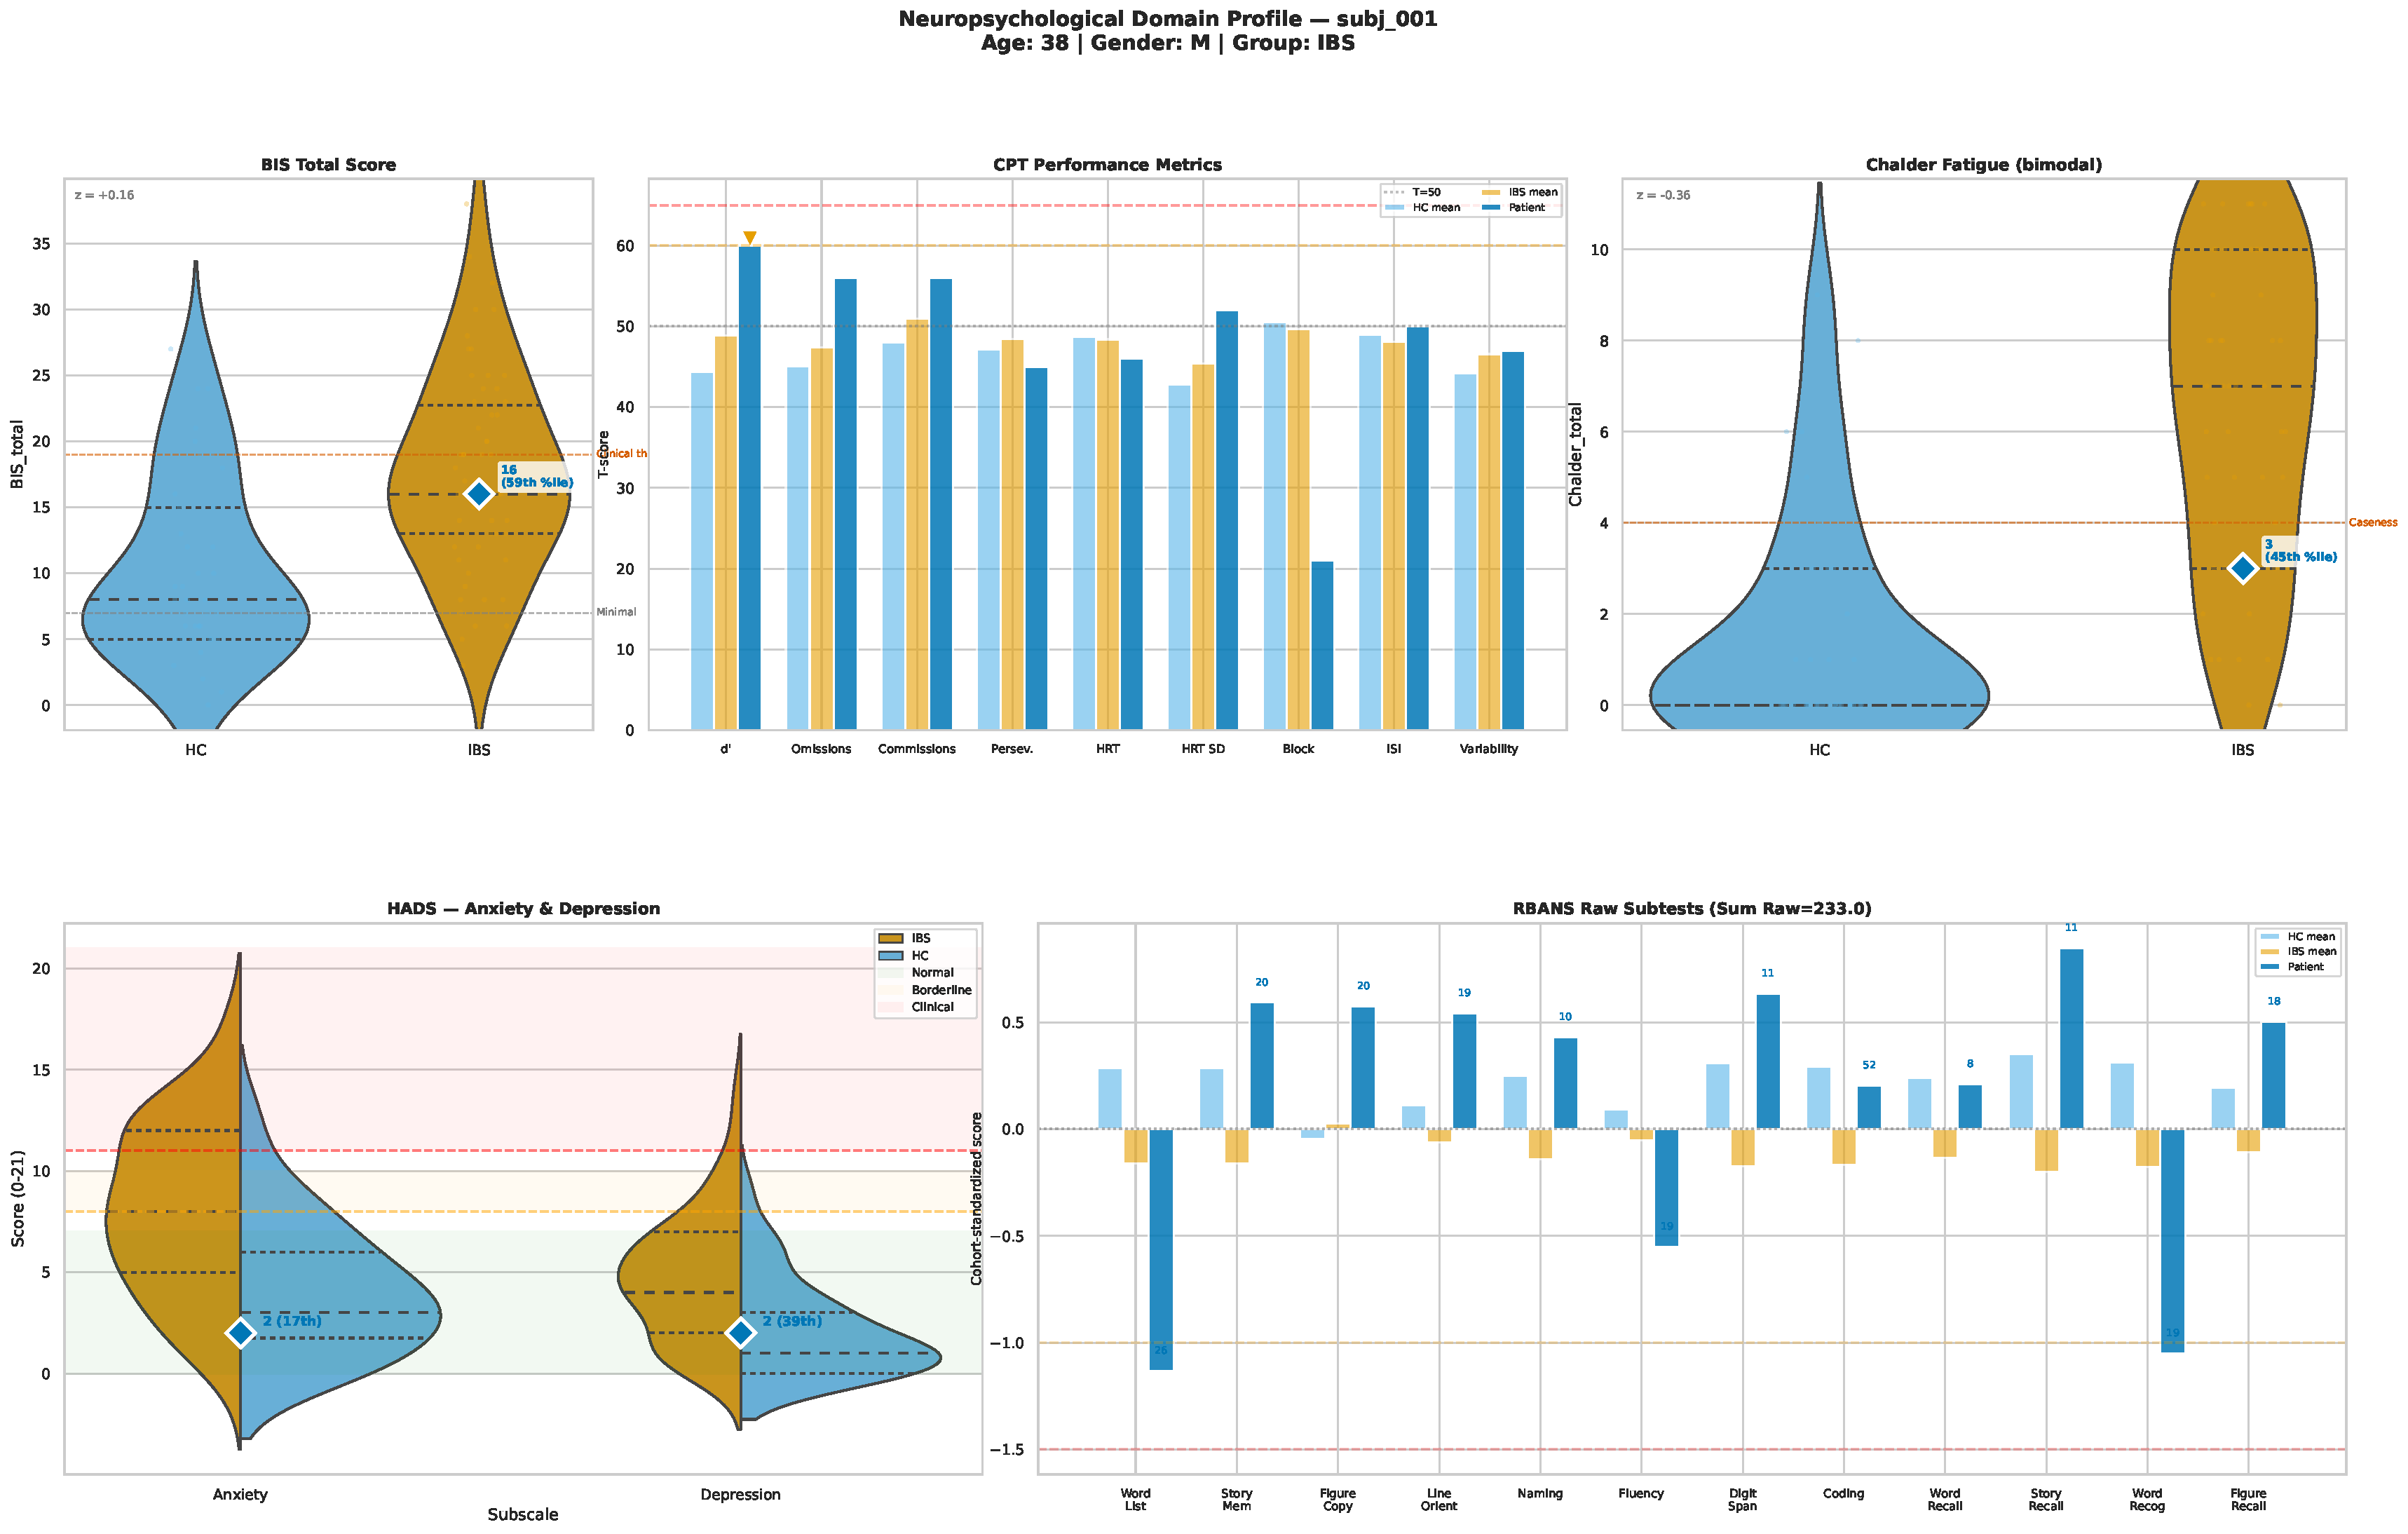
\includegraphics[width=\textwidth]{../output_subj/subj_001/subj_001_multipanel_clinical.pdf}
\caption{\textbf{Multi-panel domain profile (clinical version) for Case~1.} Each panel shows the cohort distribution (violin plots split by IBS/HC group) with the patient's score marked as a blue diamond. \textit{Panel 1 (BIS):} Insomnia total with clinical threshold. \textit{Panel 2 (CPT):} Attention metrics with software-generated T-scores. \textit{Panel 3 (Chalder):} Fatigue with caseness threshold. \textit{Panel 4 (HADS):} Anxiety and Depression with classification zones. \textit{Panel 5 (RBANS):} Raw-subtest-derived summary composites and cohort-relative position.}
\label{fig:multipanel_example}
\end{figure}

% --- FIGURE 2: Radar plots ---
\begin{figure}[H]
\centering
\begin{subfigure}[b]{0.32\textwidth}
    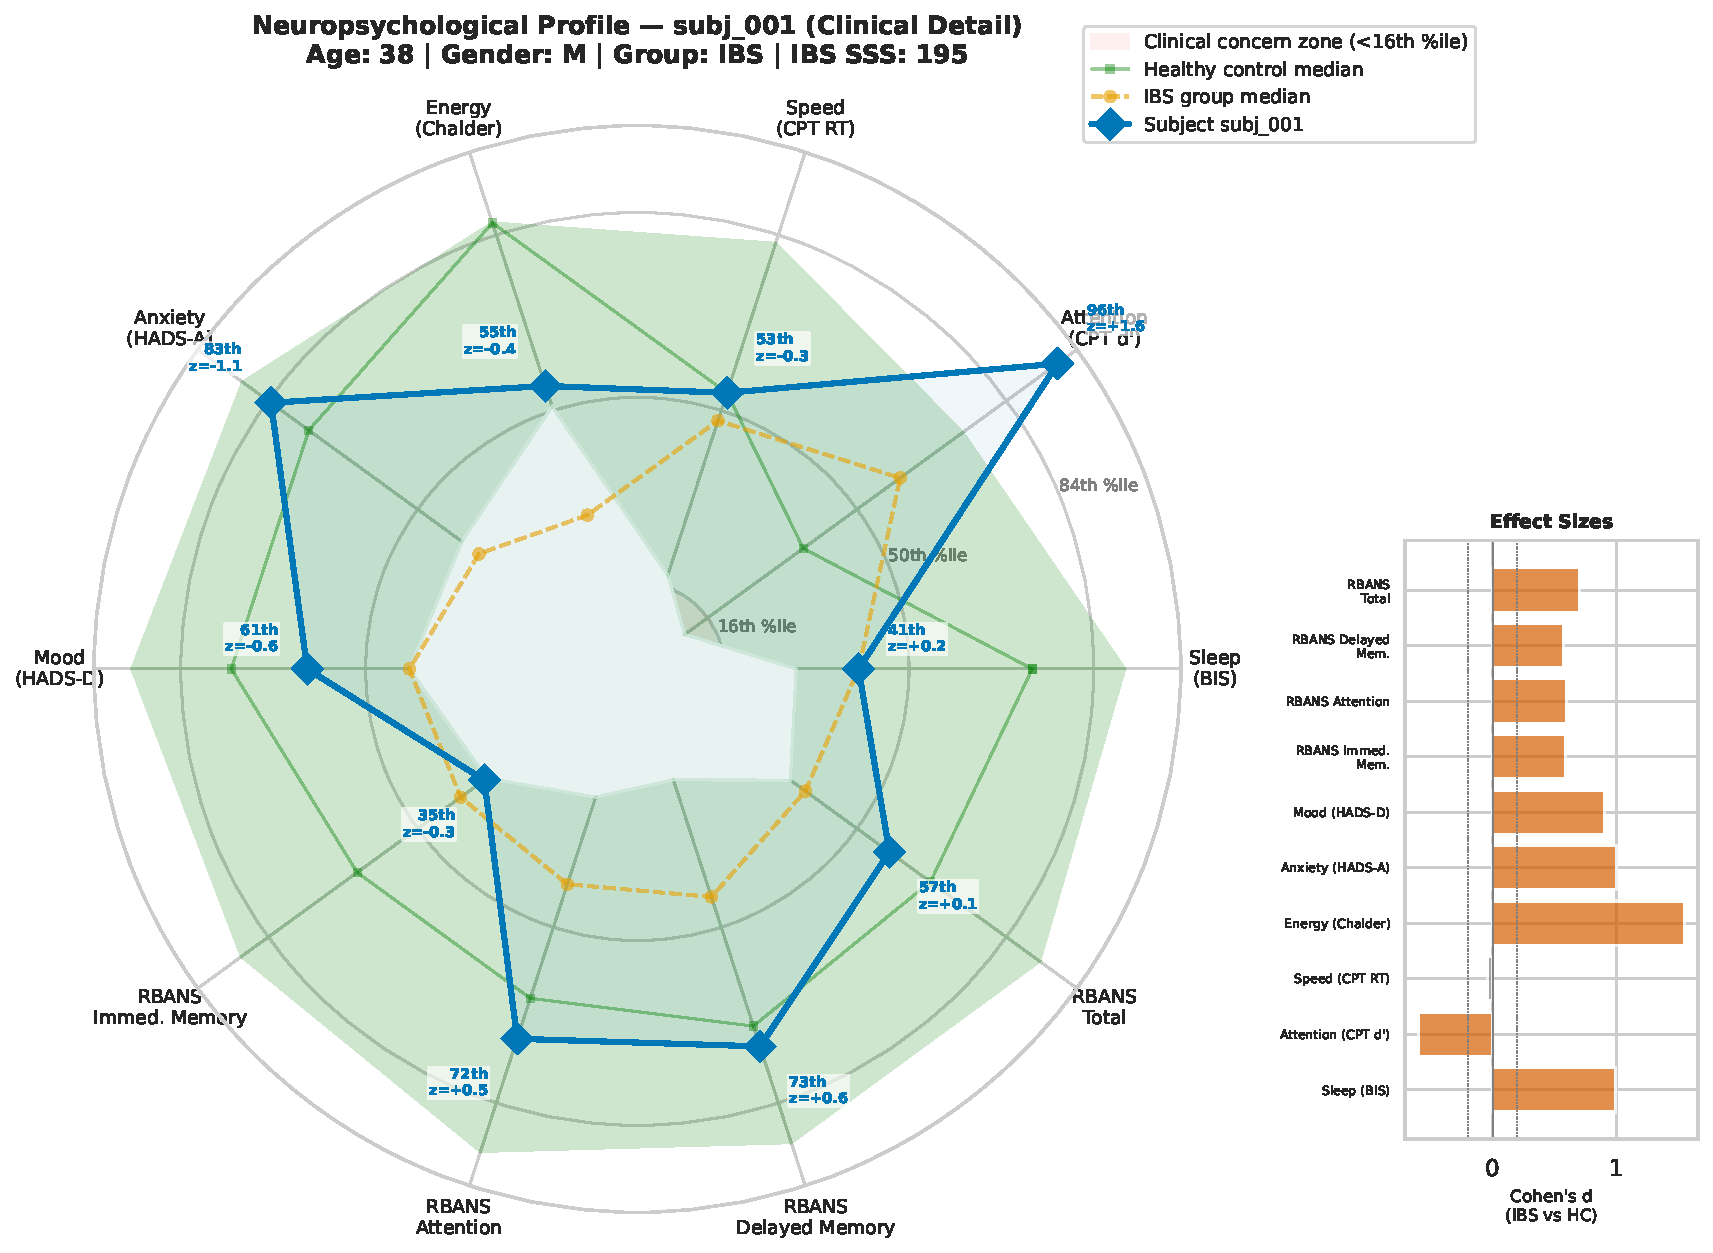
\includegraphics[width=\textwidth]{../output_subj/subj_001/subj_001_radar_clinical.pdf}
    \caption{Clinical peers}
    \label{fig:radar_clinical}
\end{subfigure}
\hfill
\begin{subfigure}[b]{0.32\textwidth}
    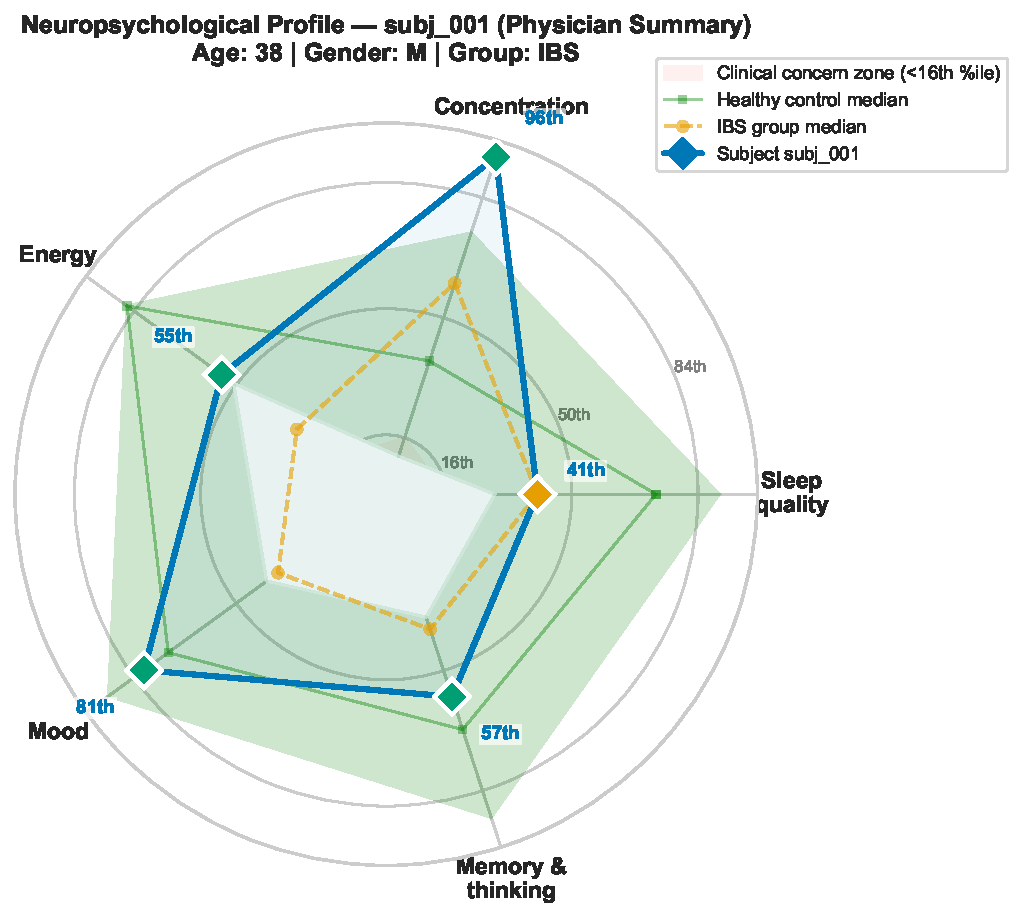
\includegraphics[width=\textwidth]{../output_subj/subj_001/subj_001_radar_physician.pdf}
    \caption{Referring physicians}
    \label{fig:radar_physician}
\end{subfigure}
\hfill
\begin{subfigure}[b]{0.32\textwidth}
    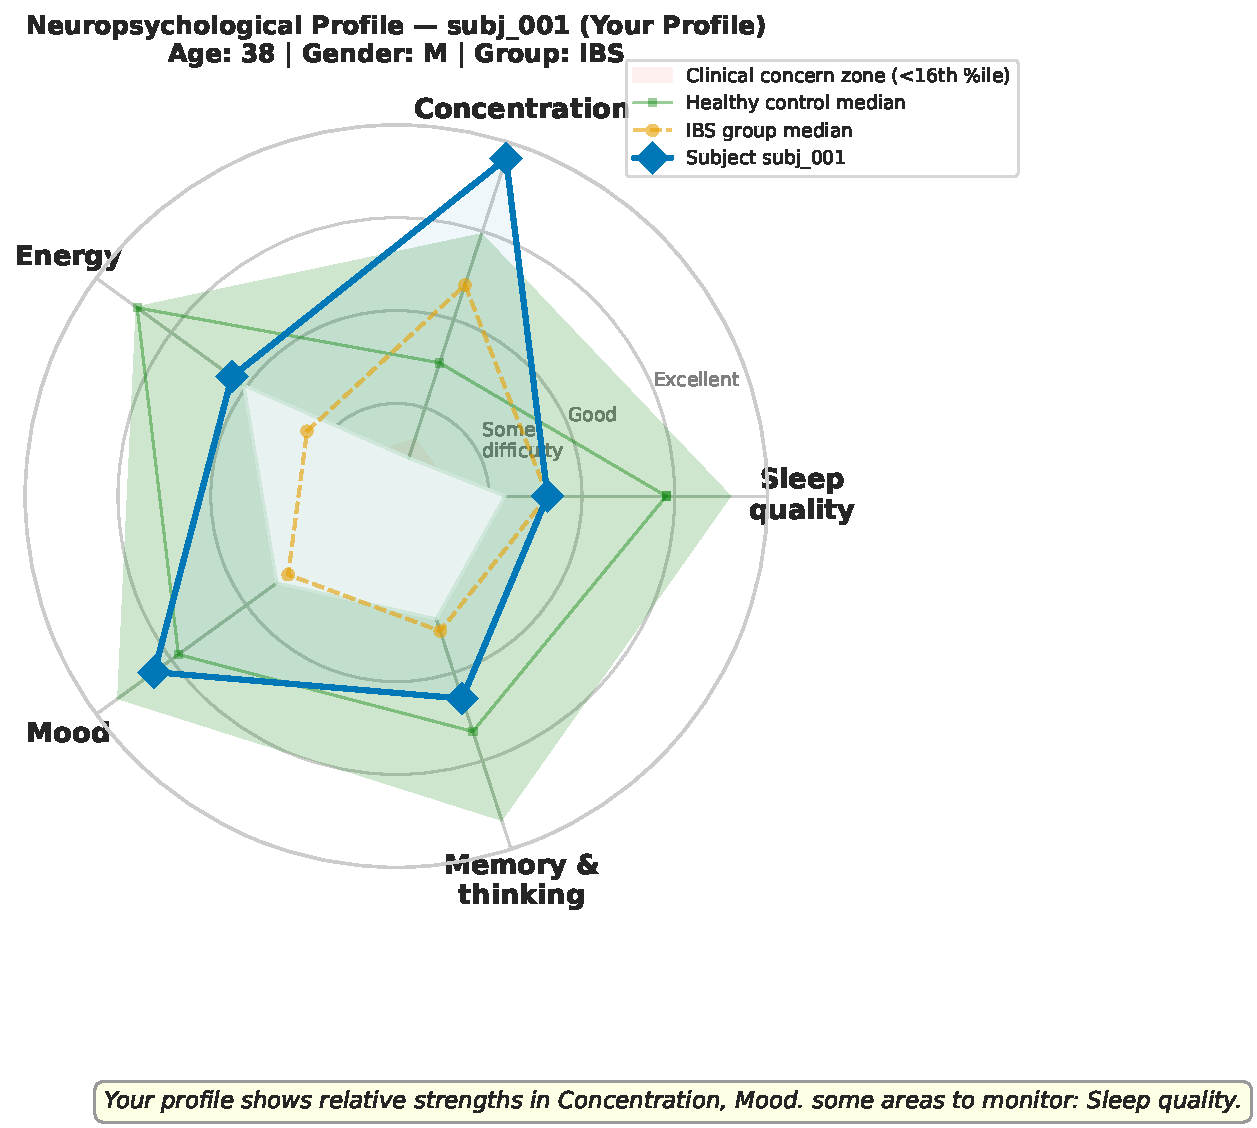
\includegraphics[width=\textwidth]{../output_subj/subj_001/subj_001_radar_patient.pdf}
    \caption{Patients \& families}
    \label{fig:radar_patient}
\end{subfigure}
\caption{\textbf{Audience-tailored radar plots for Case~1.} All three variants display the same underlying data on a normalized percentile-of-wellness scale (higher = better), but differ in level of detail and visual language. (a) The clinical version uses an expanded 10-spoke layout with $z$-score annotations and a Cohen's $d$ inset. (b) The physician version uses a compact 5-spoke layout with traffic-light coloring. (c) The patient version uses plain-language labels, qualitative anchors, and a warm palette with an interpretive sentence.}
\label{fig:radar_trio}
\end{figure}

% --- FIGURE 3: Case 2 clinical multi-panel ---
\begin{figure}[H]
\centering
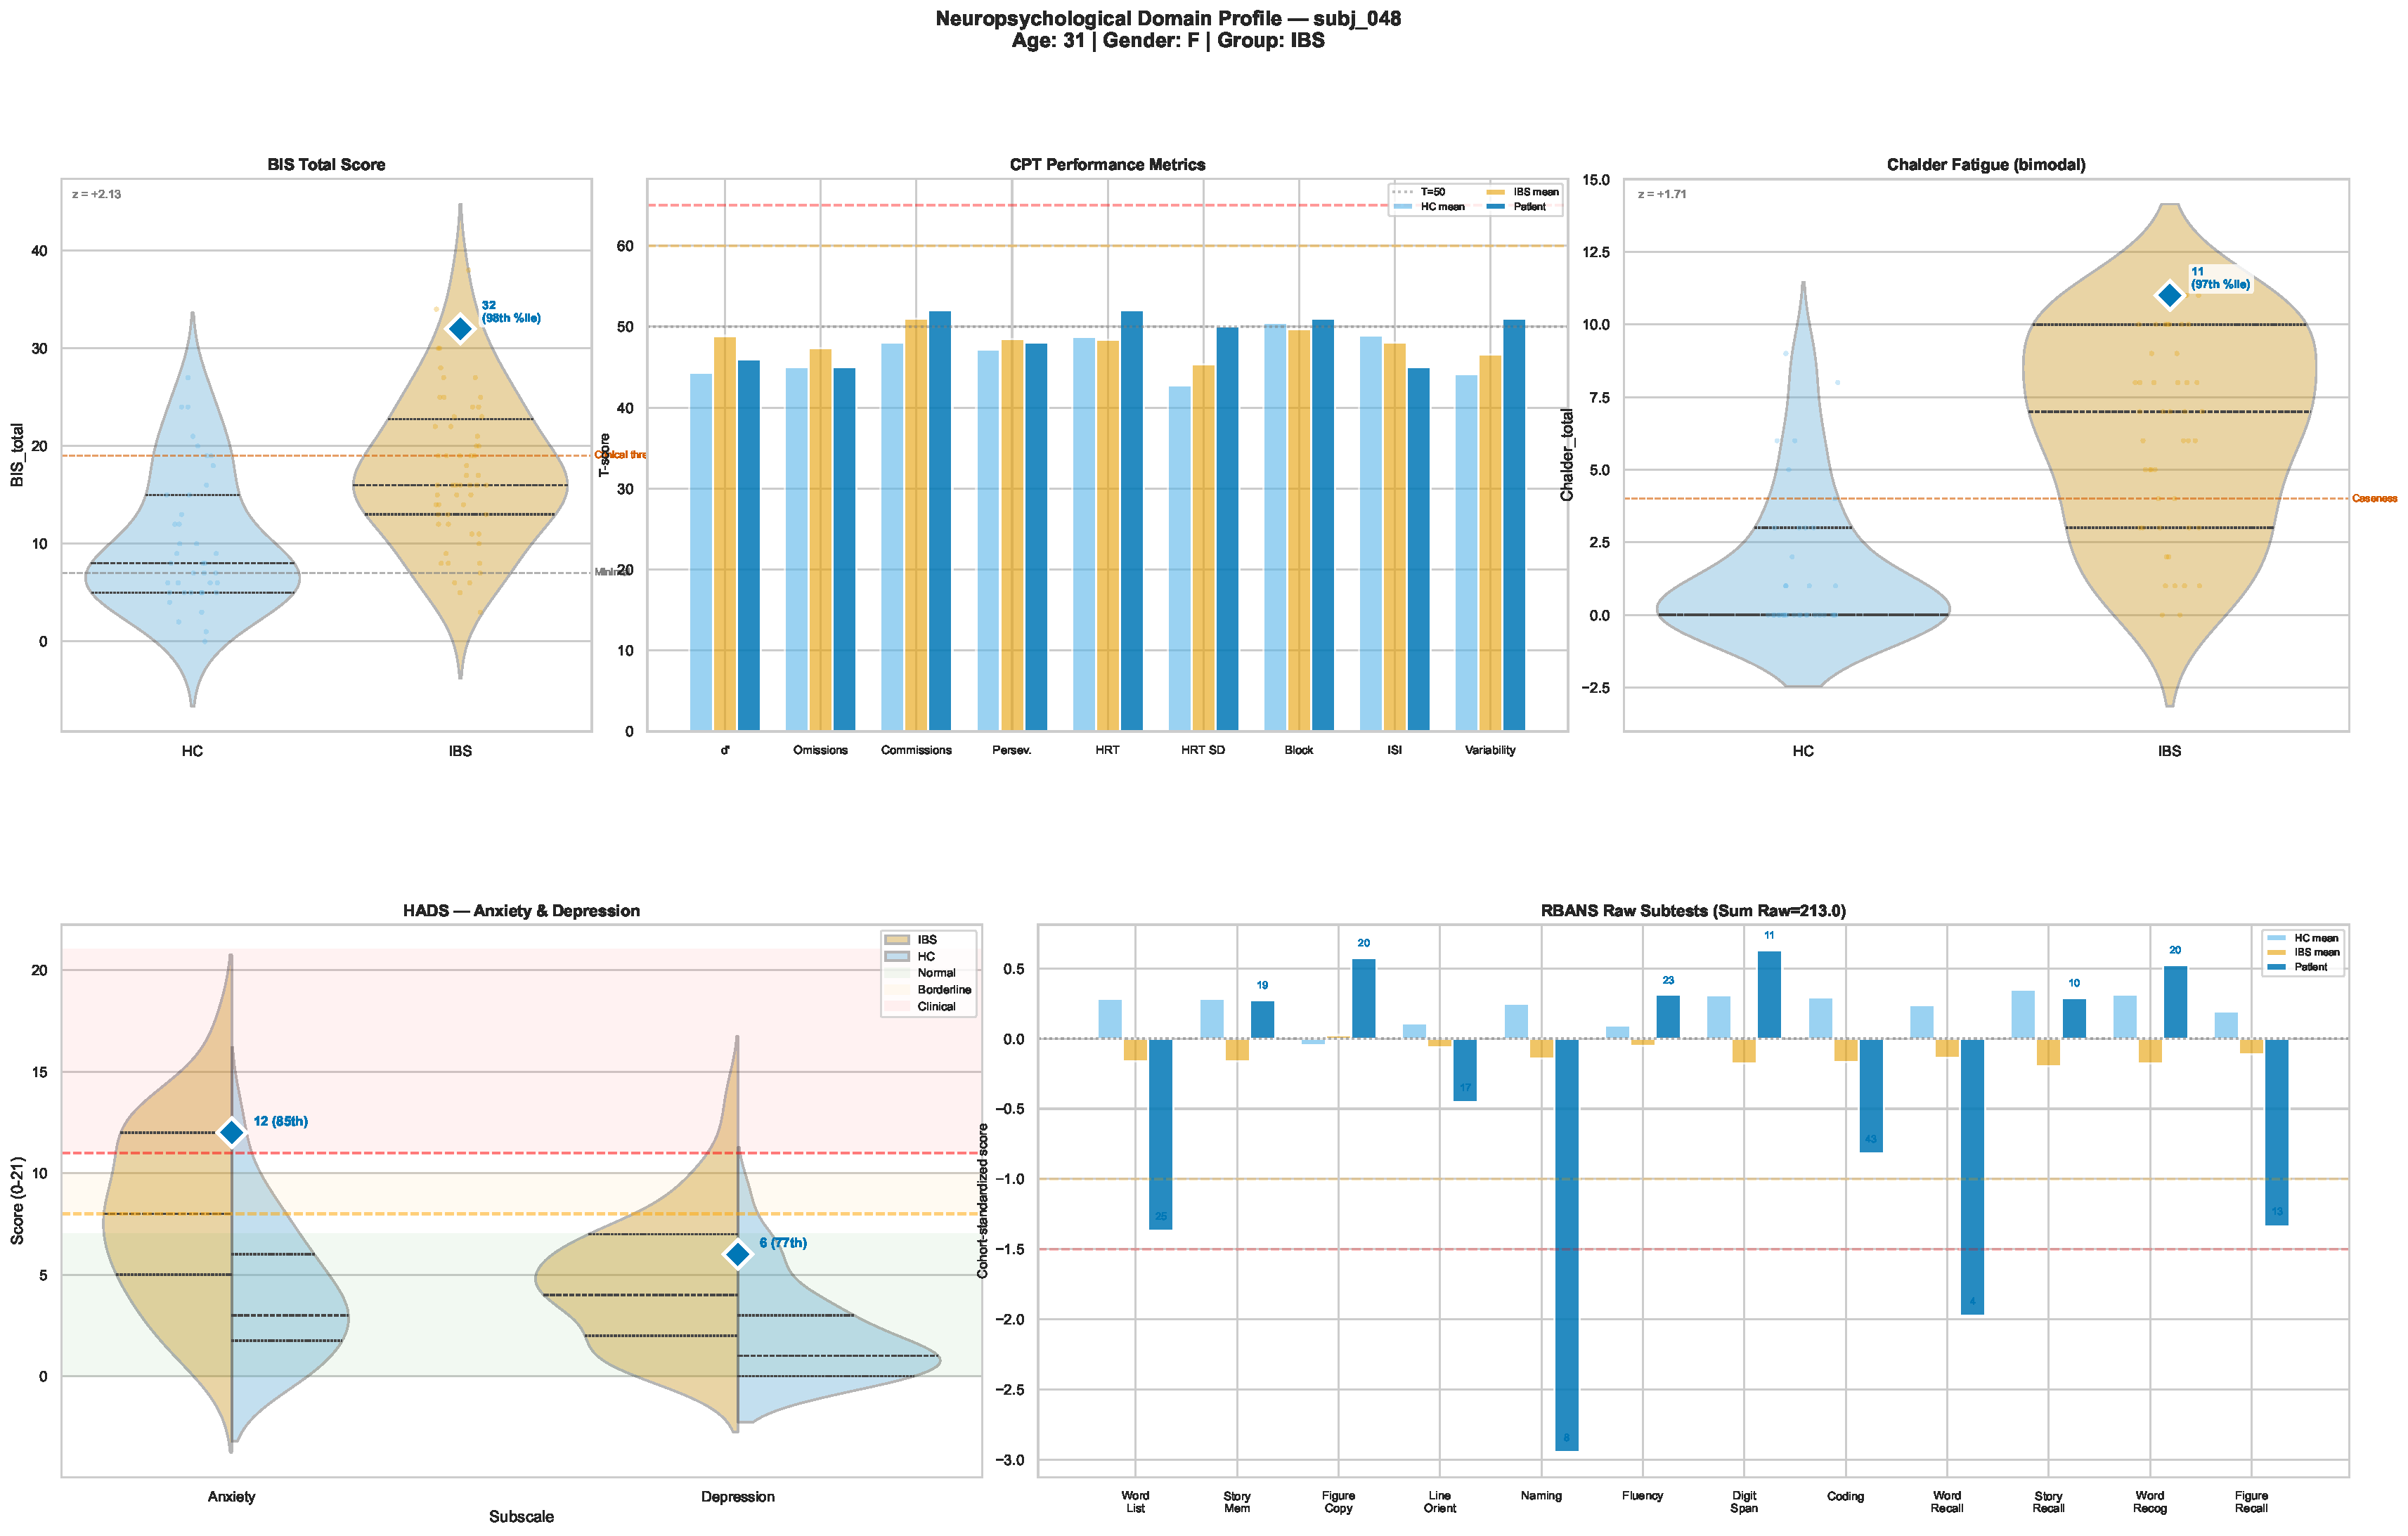
\includegraphics[width=\textwidth]{../output_subj/subj_048/subj_048_multipanel_clinical.pdf}
\caption{\textbf{Multi-panel domain profile (clinical version) for Case~2.} The pipeline output shows severe sleep disturbance, marked fatigue, clinically elevated anxiety, preserved CPT performance, and cohort-relative RBANS weakness concentrated in language and memory-related domains. As in Figure~\ref{fig:multipanel_example}, each panel plots the patient's score against the cohort distribution.}
\label{fig:case2_multipanel_clinical}
\end{figure}

% --- FIGURE 4: Case 2 radar trio ---
\begin{figure}[H]
\centering
\begin{subfigure}[b]{0.32\textwidth}
    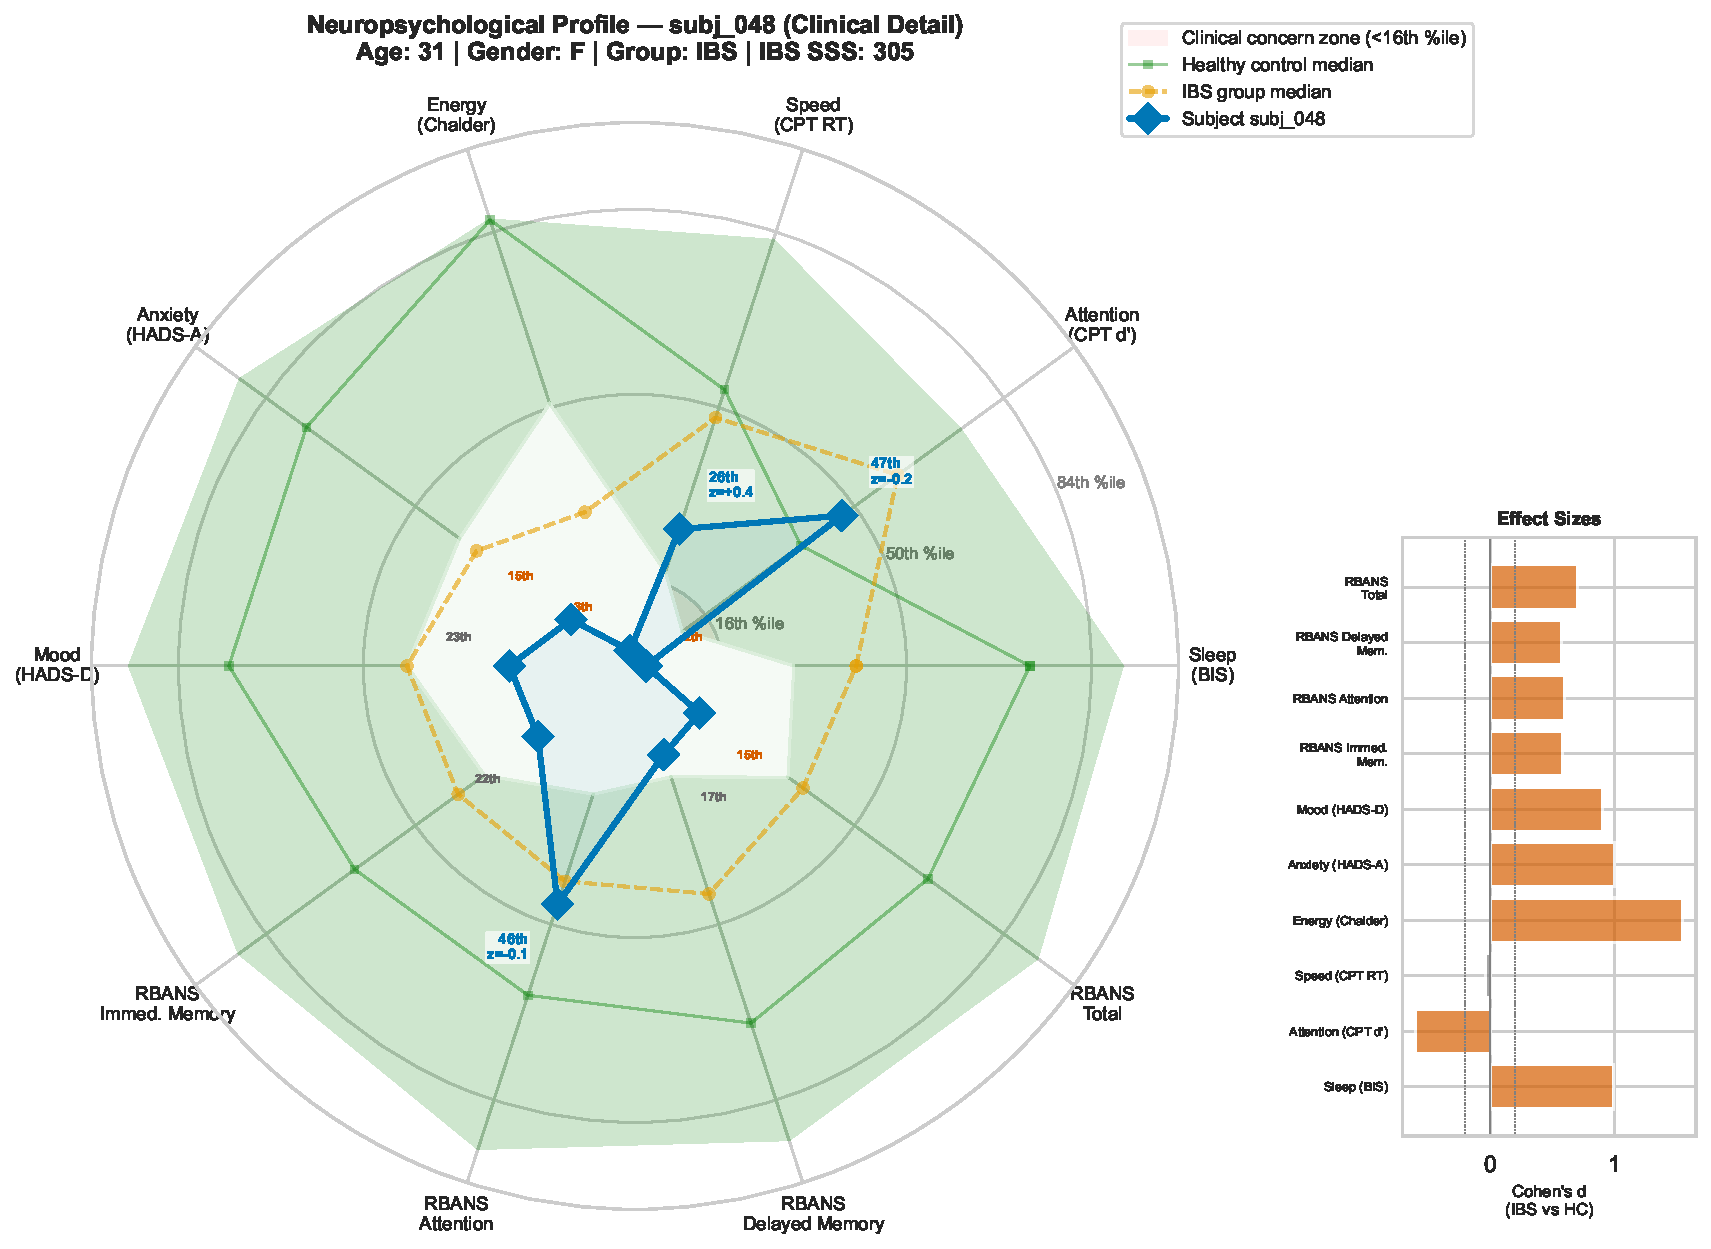
\includegraphics[width=\textwidth]{../output_subj/subj_048/subj_048_radar_clinical.pdf}
    \caption{Clinical peers}
    \label{fig:case2_radar_clinical}
\end{subfigure}
\hfill
\begin{subfigure}[b]{0.32\textwidth}
    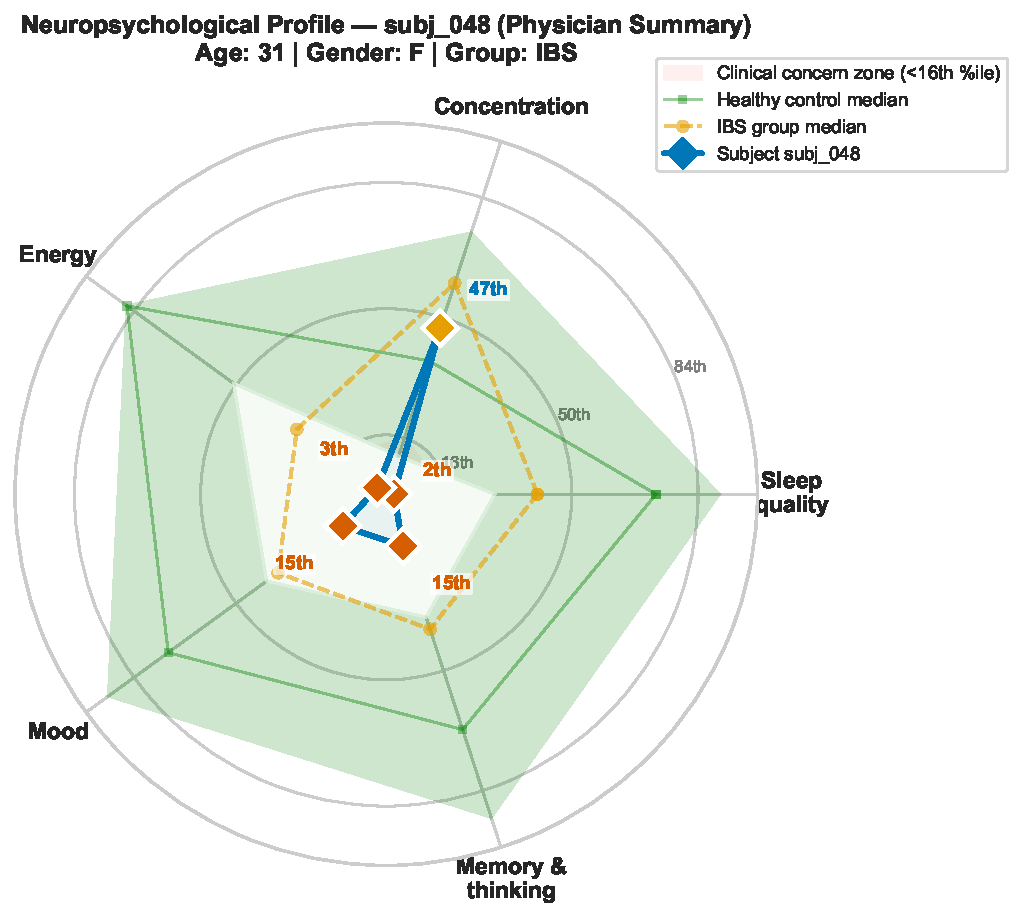
\includegraphics[width=\textwidth]{../output_subj/subj_048/subj_048_radar_physician.pdf}
    \caption{Referring physicians}
    \label{fig:case2_radar_physician}
\end{subfigure}
\hfill
\begin{subfigure}[b]{0.32\textwidth}
    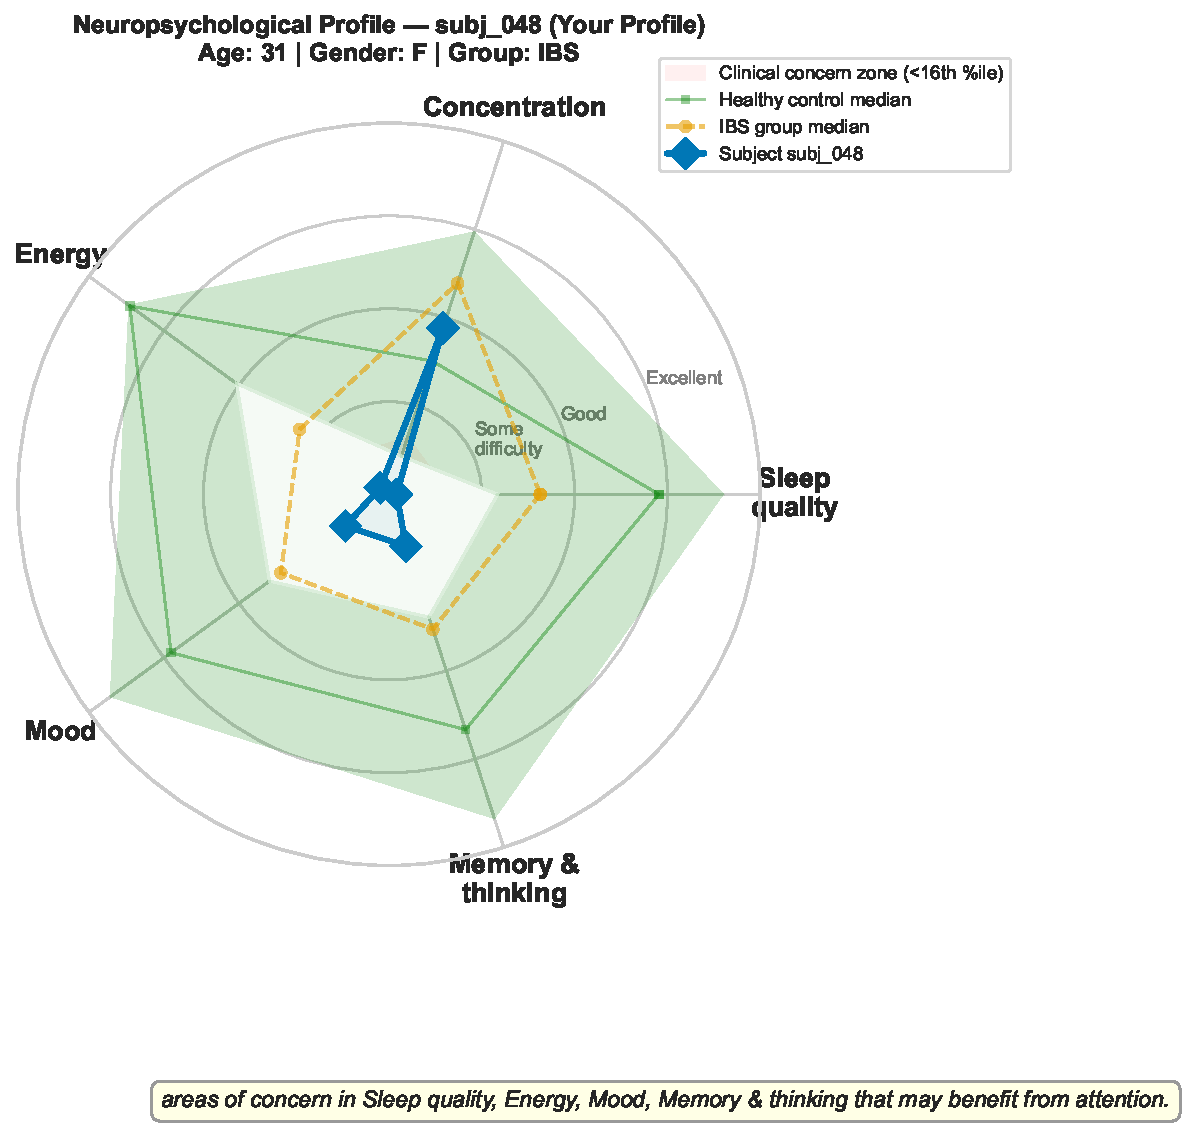
\includegraphics[width=\textwidth]{../output_subj/subj_048/subj_048_radar_patient.pdf}
    \caption{Patients \& families}
    \label{fig:case2_radar_patient}
\end{subfigure}
\caption{\textbf{Audience-tailored radar plots for Case~2.} Across all three audience versions, the updated output depicts a more globally compromised profile than Case~1, driven by severe insomnia, maximal fatigue caseness, anxiety elevation, and cohort-relative cognitive weakness, while sustained attention remains comparatively preserved.}
\label{fig:case2_radar_trio}
\end{figure}


% ============================================================================
\section{Discussion}
\label{sec:discussion}

\subsection{Summary of findings}

We developed and demonstrated a deterministic, rule-based pipeline for automated pre-examination screening in outpatient neuropsychological practice. Applied to a cohort of 105 participants (65 IBS, 40 HC), the pipeline identified clinically significant findings across five assessment domains, generated structured cross-domain reasoning chains, and produced audience-tailored outputs for clinical peers, referring physicians, and patients.

Its primary purpose is to provide the neuropsychologist with a structured synthesis of available screening data before the clinical encounter. In this way, it may reduce the time needed for pre-examination preparation and enable a more targeted clinical interview and test selection.

The main contribution of the framework is not automated diagnosis, but automated integration. Rather than merely organizing scores, the pipeline combines domain-specific findings into a preliminary clinical formulation and expresses that formulation in formats adapted to different end users. The case illustrations suggest that this approach can differentiate between relatively circumscribed and broader multi-domain profiles while also making explicit where subsequent clinician review remains essential.

\subsection{Relation to prior work}

Traditional template-based systems can populate summaries with scores \citep{Postal2018ReportWriting} but typically provide more limited support for cross-domain reasoning \citep{Donders2020}. The present framework was designed to address that gap by structuring the pre-examination synthesis itself rather than only the reporting of individual test results.

A central feature of the pipeline is the eight-step reasoning chain, which mirrors the sequence of integrative judgments clinicians make when reviewing screening data. Rather than listing isolated elevations, it links findings across domains and generates clinically plausible hypotheses about how sleep, fatigue, emotional distress, sustained attention, and broader cognition may interact. In this sense, the framework aims to support both interpretation and communication.

The deterministic architecture is important in this context. Clinicians need to understand \textit{why} a tool generated a particular interpretation, and to be able to challenge it when the clinical picture calls for it. Because every classification, flag, reasoning step, and recommendation traces back to an explicit rule, the pipeline offers transparency, reproducibility, and auditability. This is a practical advantage in clinical neuropsychology, where interpretive judgment is itself a core professional competency and where opaque generative output would be difficult to justify clinically \citep{Ji2023, DeRightPuente2026, Bhayana2024}.

\subsection{Clinical implications}

From a workflow perspective, the pipeline is best understood as a structured briefing tool for the pre-examination phase. In many outpatient services, patients or families already provide questionnaires or background information before the appointment \citep[e.g.,][]{KingsCollegeNeuropsychology2026, StanfordNeuropsychologyForms2026}. The present framework extends that workflow by automatically integrating the available screening data into a cross-domain summary before the first face-to-face encounter. Instead of reviewing separate forms manually at the start of the consultation, the clinician receives a synthesized overview of flagged areas, possible cross-domain interactions, and preliminary next-step suggestions.

This may have several practical benefits. The screening summary may help clinicians prioritise patients by identifying those with multi-domain elevations, may help guide the selection of follow-up instruments, and may serve as a discussion aid during the clinical interview. Because the pipeline applies the same published cutoffs and decision rules across patients, it may also reduce some of the inconsistency that can arise when clinicians review intake material using memory or idiosyncratic judgment alone. In multidisciplinary settings, the standardized output may additionally help clarify where initial clinical attention is best directed and may serve as a starting point for later documentation \citep{Postal2018ReportWriting}.

The cross-domain component is particularly relevant to neuropsychological practice. Its purpose is not to infer causality autonomously, but to highlight clinically meaningful constellations of findings that might otherwise remain fragmented across separate instruments. In the present cohort, this was useful for drawing attention to recurring patterns spanning sleep, fatigue, mood, and cognition. Such outputs are best understood as hypothesis-generating rather than definitive; they may help orient interview focus and test planning, but they still require clinical verification during the subsequent assessment.

The audience-tailored outputs address a related practical problem. Referring physicians often prefer brief, targeted summaries, whereas patients and family members benefit from more accessible language and visual presentation \citep{Postal2018ReportWriting, Postal2024, Gruters2022}. Producing such variants manually is time-consuming, and in practice many clinicians have little opportunity to generate separate summaries for different stakeholders. By producing distinct but data-equivalent outputs for clinical peers, physicians, and patients, the framework attempts to support communication without requiring the clinician to create multiple reports from scratch.

The case illustrations also clarify an important boundary condition of the framework: the pipeline produces a structured preliminary formulation, not a complete clinical interpretation. In both cases, the rule-based report identified the major domain findings and generated clinically plausible recommendations, but the subsequent clinician interpretation added inferences that were not explicitly captured by the rules alone. In Case~1, this concerned the significance of the convergent but relatively subtle pattern spanning sleep, attention, and verbal learning. In Case~2, it concerned the clinical importance of executive function as a possible moderator of response to anxiety-focused intervention.

The framework is therefore best understood as clinician-supervised decision support. Rules encode population-level evidence and predefined thresholds, whereas a skilled neuropsychologist integrates contextual factors, domain knowledge, clinical experience, and the patient's own account of difficulties. The pipeline does not diagnose and does not interact with patients; all outputs require professional review and may need to be modified when factors such as language, education, culture, sensory limitations, or referral context alter the meaning of the data. In this respect, the framework may extend efficiency and consistency while preserving the neuropsychologist's interpretive authority \citep{LundervoldAJ2025}.

\subsection{Limitations}

Several limitations should be acknowledged. The present study is a single-cohort, cross-sectional proof of concept based on a specific instrument battery (BIS, CPT-3, Chalder, HADS, RBANS), and extension of the framework to other batteries or clinical populations would require reconfiguration of cutoffs, variable mappings, and domain-specific logic. In addition, the validation reported here concerns computational accuracy and output completeness rather than formal clinical validity. Further work comparing pipeline-generated reports with clinician-written reports, using blinded expert ratings, is needed before broader implementation can be considered.

The interpretive scope of the framework is also bounded by the structure of its reasoning rules. The cross-domain engine generates clinically plausible hypotheses by identifying predefined constellations of findings, but it does not establish causal relationships and its outputs therefore require clinical evaluation and, where necessary, revision during the subsequent assessment. Moreover, the cohort-relative percentiles are based on $N = 105$, and the RBANS summaries are cohort-standardized rather than norm-corrected, which limits interpretive precision. Finally, the full pre-examination workflow envisioned by the framework was not achievable within the design of the present study. Although digital and remotely administered cognitive tools are already available in some settings, the present dataset required clinic-based collection of CPT-3 and RBANS data. The study also did not examine usability, accessibility, or equity, and it is unknown how the pipeline's outputs would perform for patients with limited digital access, language barriers, low health literacy, or disability-related access needs.

\subsection{Future directions}

Future work should address both clinical translation and further development of the framework. One important direction is to examine how the pipeline performs when paired with cognitive assessment tools that allow a larger proportion of the screening profile to be collected before the first clinic visit. Another is longitudinal application, as repeated processing of patient data could support structured monitoring of symptom change and treatment response over time. Because the pipeline is modular, it may also be extended to additional neuropsychological instruments and clinical populations, allowing evaluation of how well the present reasoning logic generalizes across assessment contexts.

Equally important will be studies of usability and implementation in routine care. Evaluation involving neuropsychologists, referring physicians, and patients is needed to determine whether the audience-tailored outputs improve examination planning, clinical communication, and workflow efficiency in practice. Such work should explicitly test performance across patients with differing language backgrounds, levels of digital access, health literacy, and disability-related needs, and should examine whether the audience-tailored outputs are accessible and meaningful to the groups they are intended to serve. In the longer term, integration with electronic health record systems may support use within ordinary clinical workflows, provided that transparency, governance, and professional accountability remain central.


\section{Conclusions}
\label{sec:conclusion}

The present study introduces a proof-of-concept framework for automated pre-examination screening in outpatient neuropsychological practice. Within the limits of the present dataset and rule set, the deterministic pipeline identified clinically relevant findings, generated structured cross-domain hypotheses, and produced audience-tailored outputs for different stakeholders. The framework is intended to support, rather than replace, neuropsychological judgment, and its deterministic architecture offers transparency, auditability, and reproducibility. At the same time, it should be regarded as an initial demonstration rather than as a fully validated model for routine clinical use. Its eventual clinical value will depend on formal validation, usability testing, equitable implementation, and careful integration with assessment workflows.


% ============================================================================
% ACKNOWLEDGMENTS
% ============================================================================
\section*{Acknowledgments}

The authors thank the participants in the Bergen Brain--Gut--Microbiota study for their contributions. This work was supported by the University of Bergen. Financial support: The original data collection (B-BGM project) was funded by the Research Council of Norway (grant ID FRIMED-BIO276010), Helse Vest's Research Funding (grant ID HV912243), the Trond Mohn Research Foundation (grant number BFS2018TMT0), and by The Research Council of Norway (project number 294594). The pipeline was developed using open-source Python tools and \LaTeX, and was co-authored with AI assistance (Claude Opus 4.6, Anthropic, accessed via the Cursor IDE [\url{https://cursor.com}], February 2026). The AI coding assistant contributed to writing the Python code, designing the clinical decision rules, authoring the narrative text templates, implementing the visualizations, and drafting portions of the manuscript text for language, clarity, and consistency. All AI-generated content was reviewed, verified, and edited by the authors. The deterministic pipeline uses no AI models at runtime.

\section*{Conflict of Interest}

The authors declare no conflicts of interest.

\section*{Data Availability Statement}

The cohort dataset contains clinical neuropsychological data collected under ethics approval and is not publicly available due to participant confidentiality and ethics approval conditions. Data may be made available upon reasonable request to the corresponding author, subject to institutional data sharing agreements. The pipeline source code and anonymised example outputs are openly available at \url{https://github.com/arvidl/AI-driven-neuropsych}. The complete audience-tailored reports for the two case illustrations are provided as Supplementary Material~S2 and~S3.

% ============================================================================
% SUPPLEMENTARY MATERIALS
% ============================================================================
\section*{Supplementary Material}

Supplementary Material~S1 (\texttt{supplementary\_methods.pdf}) contains the prompt-development and rule-specification materials. It includes the complete system prompt specification used as the design brief during AI-assisted development: the five assessment domains, visualization designs, audience-tailored output variants, and the structured JSON output format. The system prompt is not fed to any model at runtime. S1 also provides a transparent account of AI's role in the project (development time vs.\ runtime), followed by the complete set of explicit decision rules: classification rules for all five instruments with published cutoff sources (including the eight-step reasoning chain protocol), all cross-domain pattern detection rules with trigger conditions and mechanistic interpretations, the conditional logic for each reasoning-chain step, all recommendation generation rules, and decision-tree diagrams and flowcharts.

Supplementary Material~S2 (\texttt{case\_1\_report.pdf}) provides the complete audience-tailored pipeline report for Case~1. Supplementary Material~S3 (\texttt{case\_2\_report.pdf}) provides the corresponding report for Case~2.

% ============================================================================
% References
% ============================================================================
\clearpage
\begingroup
\small
\setstretch{1.05}
\raggedright
\sloppy
\printbibliography
\endgroup

\end{document}
